% file: Generation_proc.tex
% date: 11/05/2020
% author: Enzo MEDINA emedina@enseirb-matmeca.fr
%         Mathieu BRASSART mbrassart001@enseirb-matmeca.fr
%         Léna HEREAU   phereau@enseir-matmeca.fr
%         Killian DIEU  kdieu@enseirb-matmeca.fr


\documentclass[a4paper]{article}

\usepackage[utf8]{inputenc}
\usepackage[french]{babel}
\usepackage{graphicx}
\graphicspath{{./graphic/}}
\usepackage{subcaption}
\usepackage{amsmath, amssymb}
\usepackage[left=3cm,right=3cm,top=2cm,bottom=2cm]{geometry}
\usepackage{url}

\usepackage[T1]{fontenc}
\usepackage{fullpage}
\usepackage{color}
\usepackage{listings}
\usepackage{algorithm}
\usepackage{algorithmic}

\renewcommand{\lstlistingname}{Algorithme}

\definecolor{codegreen}{RGB}{32, 124, 47}

\lstset{
  aboveskip=3mm,
  belowskip=-2mm,
  backgroundcolor=\color{white},
  basicstyle=\footnotesize,
  breakatwhitespace=false,
  breaklines=true,
  captionpos=b,
  commentstyle=\color{codegreen},
  deletekeywords={...},
  escapeinside={\%*}{*)},
  extendedchars=true,
  framexleftmargin=16pt,
  framextopmargin=3pt,
  framexbottommargin=6pt,
  frame=tb,
  keepspaces=true,
  keywordstyle=\color{blue},
  language=C,
  literate=
  {²}{{\textsuperscript{2}}}1
  {⁴}{{\textsuperscript{4}}}1
  {⁶}{{\textsuperscript{6}}}1
  {⁸}{{\textsuperscript{8}}}1
  {€}{{\euro{}}}1
  {é}{{\'e}}1
  {è}{{\`{e}}}1
  {ê}{{\^{e}}}1
  {ë}{{\¨{e}}}1
  {É}{{\'{E}}}1
  {Ê}{{\^{E}}}1
  {û}{{\^{u}}}1
  {ù}{{\`{u}}}1
  {â}{{\^{a}}}1
  {à}{{\`{a}}}1
  {á}{{\'{a}}}1
  {ã}{{\~{a}}}1
  {Á}{{\'{A}}}1
  {Â}{{\^{A}}}1
  {Ã}{{\~{A}}}1
  {ç}{{\c{c}}}1
  {Ç}{{\c{C}}}1
  {õ}{{\~{o}}}1
  {ó}{{\'{o}}}1
  {ô}{{\^{o}}}1
  {Õ}{{\~{O}}}1
  {Ó}{{\'{O}}}1
  {Ô}{{\^{O}}}1
  {î}{{\^{i}}}1
  {Î}{{\^{I}}}1
  {í}{{\'{i}}}1
  {Í}{{\~{Í}}}1,
  morekeywords={*,...},
  numbers=left,
  numbersep=10pt,
  numberstyle=\tiny\color{black},
  rulecolor=\color{black},
  showspaces=false,
  showstringspaces=false,
  showtabs=false,
  stepnumber=1,
  stringstyle=\color{black},
  tabsize=4,
  title=\lstname,
}


\begin{document}


\begin{titlepage}
    \begin{sffamily}
    \begin{center}
    
    ~\\[1.5cm]
    \textsc{\LARGE ENSEIRB-MATMECA}\\[1.5cm]
    
    \textsc{\Large Filière Informatique - 1ère année}\\[2cm]
    
    
        % Title
        \hrulefill \\[0.4cm]
    { \Huge \bfseries Rapport de projet \\[0.4cm] }
    { \huge \bfseries Quoridor \\[0.4cm] }
     \hrulefill \\[2cm]
     
     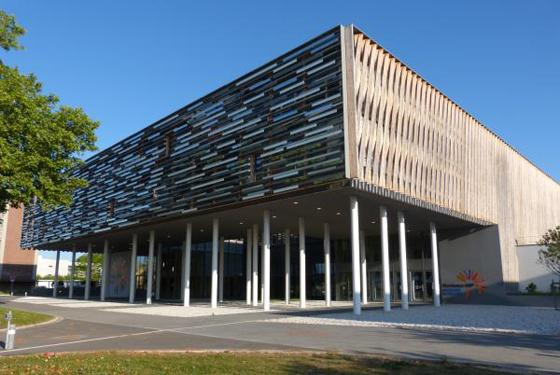
\includegraphics[scale=0.6]{rapport/enseirb_matmeca.jpg} \\[1cm]
     
    % Authors
    \begin{minipage}{0.4\textwidth}
      \begin{flushleft} \large
         \emph{Auteurs :} \\
        Enzo MEDINA\\
        Mathieu BRASSART \\
        Léna HEREAU \\
        Killian DIEU \\
      \end{flushleft}
    \end{minipage}
    \begin{minipage}{0.4\textwidth}
      \begin{flushright} \large
        \emph{Encadrants :} \\
        M. RENAULT\\
        M. POPOV \\
      \end{flushright}
    \end{minipage}
    
     ~\\[1.5cm]
    {\large 9 Mars 2021 — 21 Mai 2021}
    
    \end{center}
    \end{sffamily}
\end{titlepage}


\tableofcontents

\newpage

\section{Introduction}

\paragraph{}
Le but de ce projet\cite{sujet} est de recréer le jeu de plateau Quoridor et de pouvoir simuler des parties entre deux joueurs en langage C. L'implémentation de la boucle de jeu, aussi appelée \textbf{serveur}, doit être compatible avec n'importe quelle bibliothèque dynamique de joueur. Ces joueurs seront confondus avec le terme de \textbf{client}.

\paragraph{}
Étant un projet de programmation C, d'importantes notions du cours\cite{cours} ont été gardées en tête pour établir une programmation en fichiers séparés, une compilation automatique avec l'outil \texttt{make}, la génération de couverture ainsi que la création de tests pertinents tout le long du projet.

\subsection{Règles du jeu}
\paragraph{}
Quoridor est un jeu de plateau à deux joueurs, où ces deux joueurs s'affrontent sur une grille carrée où chaque case est séparée par des petits espaces creux, les arêtes, pour pouvoir y placer des murs (coupant nécessairement deux arêtes). Le but du jeu est d'arriver de l'autre côté du plateau en premier. Chaque joueur commence à une de ses positions de départs, c'est-à-dire sur une des cases du bord du plateau de son côté, et tour à tour les joueurs peuvent décider d'avancer d'une case ou de placer un mur, permettant ainsi de bloquer certains mouvements.

\subsubsection{Déplacement du joueur}
\paragraph{}
Un joueur peut se déplacer d'une case dans chaque direction, en utilisant le voisinage de von Neumann\cite{voisinage}. Cependant, pour pouvoir faire ce déplacement, il est impératif qu'aucun mur ou bordure du plateau ne bloque la route du joueur. Trois déplacements supplémentaires s'ajoutent à la liste des quatre déplacements élémentaires. Si le joueur fait face à son opposant, il peut, au lieu d'être bloqué par ce dernier, sauter par dessus lui et ainsi se déplacer de deux cases au lieu d'une. Si un mur se trouve derrière l'opposant, un saut en diagonal est autorisé, s'il n'est pas lui aussi bloqué par un mur. Ces déplacements sont visibles plus clairement en figures~\ref{fig:valid_pos1} et~\ref{fig:valid_pos_ennemy}.

\subsubsection{Placement d'un mur}
\paragraph{}
Un joueur peut décider de placer un mur sur le plateau afin de limiter le nombre de déplacements possible lors de la partie. Placer un mur nécessite plusieurs conditions. Tout d'abord, le joueur doit encore avoir des murs à disposition. Ensuite, le joueur peut poser un mur uniquement sur une paire d'arêtes du plateau. De plus, un mur ne peut pas être posé s'il croise un autre mur du plateau. Enfin, le mur posé doit laisser au moins un chemin possible pour chaque joueur entre son pion et une de ses positions gagnantes. Ces placements sont visibles plus clairement en figures~\ref{fig:valid_walls_trouble},~\ref{fig:check_path1} et~\ref{fig:check_path2}.

\clearpage
\section{Graphes de jeu}

\subsection{Gestion du plateau}
\paragraph{}
L'implémentation des graphes de jeu se fait par la bibliothèque \texttt{GSL} d'après les caractéristiques imposées par le sujet, en utilisant des matrices creuses en guise de matrices d'adjacence d'un graphe. Pour chaque coordonnées \texttt{(i,j)} sur le graphe, l'entier associé correspond au type de liaison entre le sommet~\texttt{i} et le sommet~\texttt{j}. La valeur $0$ signifie que le sommet~\texttt{i} n'est pas voisin avec le sommet~\texttt{j}. Une valeur comprise entre $1$ et $4$ signifie que le sommet~\texttt{j} est respectivement au nord, au sud, à l'ouest ou à l'est du sommet~\texttt{i}.

\paragraph{}
Un tel choix de représentation rend possibles des incohérences sur le graphe, car l'ajout d'un entier au mauvais endroit peut donner des situations impossibles physiquement (deux sommets voisins dans le graphe alors qu'à plusieurs cases d'écart dans la réalité). De plus, il apparaît nécessaire de coder une interface pour l'utilisation de cette matrice afin de ne pas se reposer sur la numérotation des sommets - qui pourrait être différente sur d'autres serveurs. Par l'implémentation de notre fichier \texttt{graph\_modif.h}, nous gagnons ainsi en généralisation dans le code. Ainsi donc, on obtient en partant d'une matrice d'adjacence (Figure~\ref{fig:matrice}) un graphe lisible (Figure~\ref{fig:graphe}). \\

\begin{figure}[ht]
    \centering
    \begin{subfigure}{.5\textwidth}
        \centering
        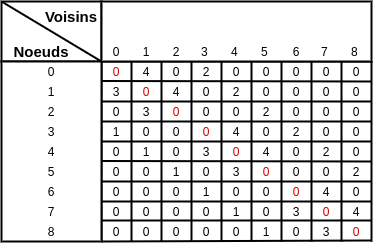
\includegraphics[scale=0.65]{rapport/matrice_adjacence.png}
        \caption{Matrice d'adjacence d'un graphe 3x3}
        \label{fig:matrice}
    \end{subfigure}%
    \begin{subfigure}{.5\textwidth}
        \centering
        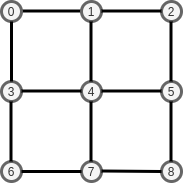
\includegraphics[scale=0.86]{rapport/graphe.png}
        \caption{Graphe d'un graphe 3x3}
        \label{fig:graphe}
    \end{subfigure}
    
    \caption{Différentes représentations d'un même plateau de jeu. La ligne $0$ en figure~\ref{fig:matrice} définit le noeud~$1$ à l'est et le noeud~$3$ au sud du noeud~$0$.}
    \label{fig:representations}
\end{figure}

\paragraph{}
Un ensemble de fonctions de \textbf{manipulation de graphe} ont ainsi été implémentées, pour que jamais nos autres fichiers n'aient à manipuler les matrices directement. Ainsi, nous avons développé des fonctions pour initialiser des graphes vides, les remplir selon les formes voulues dans le sujet (voir Figure~\ref{fig:graphshape}), ainsi que faire la copie d'un graphe ou retrouver leur taille d'origine à partir de leur nombre de sommets. Cette dernière fonction sera particulièrement utile lors de l'initialisation, car seul le graphe peut être envoyé aux joueurs, et ceux-ci doivent alors se débrouiller pour retrouver sa taille.

\begin{figure}
    \centering
    \includegraphics[width=0.9\columnwidth]{rapport/graphshape.png}
    \caption{Les différentes formes de graphes: carré, torique, haché et serpent.}
    \label{fig:graphshape}
\end{figure}

\paragraph{}
Les fonctions orientées \textbf{manipulation de joueur} contiennent elles de quoi connaître l'existence d'une case voisine dans une direction (\texttt{graph\_\_get\_neighboor}), connaître l'existence d'une arête entre deux sommets (\texttt{graph\_\_edge\_exists}), ajouter et enlever des arêtes, ainsi que gérer les positions gagnantes.

\paragraph{}
La plupart de ces algorithmes sont de simples parcours de listes, et les méthodes \texttt{void} ont été remplacées par des fonctions renvoyant des entiers indiquant si l'exécution s'est bien déroulée ou non. Ainsi, les algorithmes des joueurs peuvent par exemple tester s'ils peuvent se déplacer dans une direction en regardant le retour de la fonction de déplacement.

\subsection{Murs et affichage}
\paragraph{}
Nous avons choisi de représenter les murs par des "arêtes manquantes" au niveau du graphe principal. Un tel choix permet des manipulations plus légères, puisqu'aucun objet "mur" n'existe, mais certaines règles spéciales du jeu nécessiteront plus tard (voir section~\ref{subsect:valid_walls}) de garder une liste des murs placés sous forme d'indices de sommets. 

\paragraph{}
Un \textbf{affichage de graphe} (voir figure~\ref{fig:graphdisplay}) a de plus été ajouté, pour permettre de suivre l'avancement des parties, le retrait progressif des arêtes quand les murs sont ajoutés, et les mouvements des deux joueurs. Puisque cette fonction est implémentée avant la création de la structure \texttt{player}, les positions des joueurs doivent être données comme deux entiers représentant leur sommet. Mettre ces valeurs à -1 permet de ne pas les afficher, et d'avoir simplement un affichage du graphe.

\begin{figure}
    \centering
    \includegraphics[width=0.6\columnwidth]{rapport/graphdisplay.png}
    \caption{Affichage de fin de partie avec victoire du joueur noir (positions gagnantes rouges) sur le joueur blanc (positions gagnantes bleues)}
    \label{fig:graphdisplay}
\end{figure}

\clearpage
\section{Communication Serveur/Client}

Maintenant que nous pouvons visualiser le plateau, nous allons devoir mettre en place le serveur et les joueurs.
Dans cette partie, nous verrons comment ils sont définis. Nous étudierons ensuite les différences entre les joueurs du point de vue du serveur et des clients et finalement la communication entre le serveur et ses clients.

\subsection{Construction d'un joueur}

\subsubsection{Définition d'un joueur (Côté Client)}

Les clients ou joueurs sont définis par le fichier \fbox{player.h}. Ils doivent tous respecter les standards imposés à savoir: \\

\begin{enumerate}
    \item \textbf{Une fonction de nommage} \\
Fonction sans argument qui permet la récupération du nom du client. Cela permet de différencier les clients au delà du nom de fichier.
    \item \textbf{Une fonction d'initialisation} \\
Elle permet la création du joueur par le client. Elle prends en argument la couleur du joueur \texttt{id}, le graphe initialisé par le serveur \texttt{graph} et le nombre de murs fournis par le serveur \texttt{num\_walls}.
    \item \textbf{Une fonction de finalisation} \\
Elle permet la libération de tout les espaces alloués par le client.
    \item \textbf{La fonction de jeu} \\
La fonction de jeu permet d'obtenir, à partir du mouvement adverse, le mouvement du client. \\
\end{enumerate}

Ces fonctions seront appelées par le serveur pour exécuter les comportements clients. La façon dont sont définis les clients est parfaitement arbitraire, et ils peuvent chacun être définis de manière totalement différente sans que cela ne pose problème. Ils sont indépendants car définis en interne, c'est le serveur qui lui a une même définition pour tout les clients.

\subsubsection{Définition d'un joueur (Côté Serveur)}
Pour que le serveur gère les joueurs, on définit une structure \texttt{player} (voir Algorithme~\ref{algo:struct_player}). \\

À l'intérieur, on y définit des données essentielles au jeu telles que la couleur du joueur, l'état du plateau (\texttt{graph}), les positions du joueur et de l'adversaire, etc. 
On y ajoute également les pointeurs de fonctions (\texttt{get\_name}, \texttt{initialize}, \texttt{player\_play} et \texttt{finalize}) qui permettent au serveur d'appeler les fonctions clients. \\

\begin{lstlisting}[caption = {Structure player}, label = {algo:struct_player}, float=ht!]
      // Description player
   size_t pos; 
   size_t ennemy_pos; 
   enum color_t id;
   int first_move; 

     // Description graph
   struct graph_t * graph;
   size_t n; 
   size_t num_walls;

      // Win
   int numb_win; 
   size_t* winning_nodes;
   size_t* owned_nodes; 
    
      // Functions client
   char* (*get_name)();
   void (*initialize) (enum color_t, struct graph_t*, size_t);
   struct move_t (*player_play) (struct move_t);
   void (*finalize) (); 
\end{lstlisting}

Nos clients sont définis eux aussi avec des structures \texttt{player}. Cependant, il y a certaines différences entre la structure joueur du côté du serveur et du côté des clients, quand bien même ils utilisent la même structure. \\

\begin{itemize}
    \item \textbf{Côté serveur}
    \begin{itemize}
        \item Graphes \\
On construit un graphe central, nommé \texttt{server\_Graph}, qui représente le plateau global. Il y a uniquement un graphe qui est commun aux joueurs. On met donc à jour un seul graphe.\\
        \item Positions gagnantes des joueurs \\
On construit les positions gagnantes et les positions d'apparition pour une seule couleur. Pour le second joueur, on inverse dans la structure les positions gagnantes/d'apparitions pour éviter la duplication de tableaux. \\
        \item Fonctions de jeu \\
Le serveur a besoin des fonctions des joueurs pour faire avancer la partie de jeu. \\
    \end{itemize}
    
    \item \textbf{Côté clients}
    \begin{itemize}
        \item Graphes \\
Chaque joueur a besoin de son propre graphe pour suivre la partie et adapter sa stratégie. Les mises à jour sont effectuées pour chacun des clients. \\
        \item Positions gagnantes des joueurs \\
On construit les positions gagnantes et les positions d'apparition pour chacun des joueurs lors de l'initialisation. \\
        \item Fonctions de jeu \\
Le client a d'ores et déjà accès à ses propres fonctions, le client connaît sa stratégie, son nom, etc. Par conséquent, il n'y a pas besoin de les récupérer, les pointeurs sont tous égaux à \fbox{NULL}. \\
    \end{itemize}
\end{itemize}

\subsection{Bibliothèques de joueurs}

Pour implémenter les clients, on charge des bibliothèques dynamiques via la bibliothèque \fbox{dlfcn.h}. L'appel de la fonction \texttt{dlopen} permet l'ouverture du fichier, qu'on doit conserver ouvert jusqu'à la fin de la partie, et \texttt{dlclose} sa fermeture. On stocke alors chacune des fonctions de player.h dans les pointeurs de la structure player. Dès lors, on peut appeler les fonctions à partir du serveur pour avancer dans la partie. \\

\subsection{Communication serveur - clients}

Pour pouvoir tester et commencer de vraies parties, nous avons créé deux premiers joueurs aléatoires : \fbox{Jerry}, un joueur qui se déplace aléatoirement, et \fbox{Morty}, un joueur qui se déplace et pose des murs de manière aléatoire. Le fait de poser un mur aléatoire (et donc de modifier le graphe de façon permanente) permet d'obtenir une grande diversité de comportement et un début de partie réelle. Chaque coup joué par un joueur est défini en prenant en argument le mouvement du joueur adverse (voir Algorithme~\ref{algo:play}) pour pouvoir mettre à jour la partie. \\
\begin{lstlisting}[caption = {Prototype de la fonction \texttt{play}}, label = {algo:play}, float = h]
struct move_t play(struct move_t previous_move); 
\end{lstlisting}

Les clients et le serveur sont mis à jour de façon différentes. Du côté client, chaque joueur se met à jour et c'est en recevant par le serveur le coup joué qu'on met à jour le graphe. Le serveur lui met à jour les 2 joueurs à chaque coup joué en modifiant les valeurs de position et de position ennemie ou en coupant des arêtes uniquement sur le graphe central. \\

On spécifie les messages d'erreurs pour qu'ils indiquent si l'erreur provient du serveur ou du client ce qui permet une meilleure visualisation du problème et simplifie le débogage. Cela permet également de vérifier les cas de triches :
Le serveur vérifie systématiquement que les mouvements décidés par les joueurs sont légaux, c'est-à-dire, s'ils appartiennent aux listes de mouvements possibles définis par les fonctions \texttt{valid\_positions} et \texttt{valid\_walls}.

\section{Implémentation des coups permis}

Nous allons maintenant regarder comment nous déterminons les mouvements légaux par le biais d'une nouvelle structure, \texttt{moves\_valids}.

\subsection{Mouvements valides}

La structure \texttt{moves\_valids} contient un tableau de structure \texttt{move\_t} alloué dynamiquement de taille 5 (Il ne peut y avoir au maximum que 5 déplacements légaux pour un joueur, ce que nous explicitons au-dessous) et un entier désignant le nombre d'élément dans ce tableau (voir Algorithme~\ref{algo:valid_positions}). L'objectif étant de remplir le tableau \texttt{valid} par tout les mouvements considérés comme légaux. \\

\begin{lstlisting}[caption = {Entête de la fonction définissant les mouvements possibles}, label = {algo:valid_positions}, float = h]
struct moves_valids* valid_positions(struct player* p)
{
   struct moves_valids *global = malloc(sizeof(struct moves_valids)); 
   struct move_t *valid = malloc(sizeof(struct move_t) * 5);
   struct move_t new; 
  
...
}
\end{lstlisting}

Pour ce faire, on appelle la fonction \texttt{valid\_positions}, prenant en argument un joueur, qui définit dans un premier temps ce qu'est un mouvement de type \fbox{MOVE} (voir Algorithme~\ref{algo:move_new}). \\

\begin{lstlisting}[caption = {Définition d'un mouvement}, label = {algo:move_new}]
struct move_t new; 
  // Definitions move
new.c = p->id; 
new.t = MOVE; 
struct edge_t e = {-1, -1};
new.e[0] = e;
new.e[1] = e;  
\end{lstlisting}
\paragraph{}
Seul l'attribut \texttt{m}, correspondant à l'identité du noeud, change en fonction des noeuds. Nous cherchons à récupérer ces identités chez les points voisins accessibles en partant de la position du joueur. Pour cela, nous appelons la fonction \texttt{graph\_\_get\_neighboor}. Trois cas sont alors possibles. \\

\begin{enumerate}
    \item \textbf{Voisin non disponible} \\
L'appel de la fonction retourne \fbox{-1} ce qui signifie que le voisin en question est hors du graphe ou que l'arête joignant les deux points est coupée. Dans ce cas, nous n'ajoutons pas le noeud à la liste des mouvements autorisés.
    \item \textbf{Voisin disponible} \\
A l'inverse, ici nous trouvons le voisin supposé dans la direction étudiée. Nous l'ajoutons aux coups légaux. 
    \item \textbf{Voisin disponible ET joueur ennemi sur cette même case}. \\
Si, en revanche, le joueur adverse se trouve sur la case atteignable, alors nous devons adapter les coups légaux. Nous vérifions d'abord que dans la même direction, un noeud est atteignable. Si c'est le cas, le coup autorisé est un double saut dans ladite direction. Sinon, nous étudions les positions latérales du joueur ennemi. Nous ajoutons chaque noeud atteignable. \\
\end{enumerate}

Ainsi, par exemple, dans la figure~\ref{fig:valid_pos1}, la liste des mouvements disponibles correspond aux noeuds \texttt{(6, 11, 14)}.

\begin{figure}[h!]
    \centering
    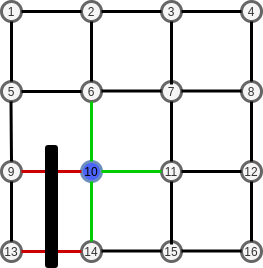
\includegraphics[scale=0.65]{rapport/valid_position1.png}
    \caption{Positions accessibles dans un cas particulier}
    \label{fig:valid_pos1}
\end{figure}

Dans le cas des figures~\ref{fig:valid_pos_e1} et \ref{fig:valid_pos_e2}, nous pouvons visualiser des exemples avec un joueur ennemi. Les positions accessibles sont respectivement \texttt{(2, 9, 11, 14)} et \texttt{(5, 7, 9, 11, 14)} en fonction de la présence du mur empêchant le double saut.

\begin{figure}[h]
    \centering
    \begin{subfigure}{.5\textwidth}
        \centering
        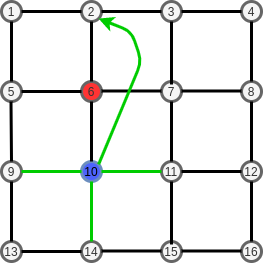
\includegraphics[width=0.75\linewidth]{rapport/valid_position_e1.png}
        \caption{Double saut possible}
        \label{fig:valid_pos_e1}
    \end{subfigure}%
    \begin{subfigure}{.5\textwidth}
        \centering
        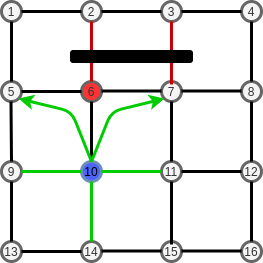
\includegraphics[width=0.75\linewidth]{rapport/valid_position_e2.png}
        \caption{Double saut impossible}
        \label{fig:valid_pos_e2}
    \end{subfigure}
    
    \caption{Positions accessibles avec un joueur ennemi en face}
    \label{fig:valid_pos_ennemy}
\end{figure}


Ainsi, nous avons pu voir par l'exemple précédent qu'il y a au maximum 5 mouvements autorisés disponibles. Les joueurs aléatoires \fbox{Jerry} et \fbox{Morty} récupèrent ces mouvements et choisissent aléatoirement l'un de ces coups.

\subsection{Murs légaux}

\subsubsection{Murs possibles}
\label{subsect:valid_walls}
La tâche est d'autant plus complexe lorsque nous souhaitons étudier les murs disponibles. En effet, s'il y a seulement 5 mouvements légaux, quelque soit l'état de la partie, il y a 32 murs disponibles pour un graphe carré initial de taille 5 par 5. C'est la fonction \texttt{valid\_walls} qui s'occupe de récupérer le nombre et la liste complète de ces murs légaux. Nous commençons par créer nos tableaux et structures (voir Algorithme~\ref{algo:valid_walls}). \\

\begin{lstlisting}[caption = {Entête de la fonction déterminant les murs légaux}, label = {algo:valid_walls}, float = h]
struct moves_valids* valid_walls(struct player* p)
{
   
      // Dynamic array Walls
   struct moves_valids* global = malloc(sizeof(struct moves_valids)); 
   struct move_t* walls = malloc(sizeof(struct move_t) * 1); 
   int size = 0; 
   int capacity = 1; 
   
...
}
\end{lstlisting}

Cette fois, nous remarquerons que la taille du tableau des \texttt{move\_t} est initialisée à 1. Nous ajoutons également deux entiers \texttt{size} et \texttt{capacity}. Ces variables nous permettront d'augmenter la taille du tableau en la multipliant par deux dès lors que \texttt{size} est égal à \texttt{capacity}. Dans ce cas, nous utilisons la fonction \texttt{realloc} qui ré-alloue de l'espace mémoire s'il y a suffisamment de place à côté du bloc mémoire du tableau ou, dans le cas contraire, qui recopie la mémoire déjà allouée et attribue un bloc mémoire plus grand. \\

Nouvelle différence également par rapport à la fonction \texttt{valid\_positions}, les murs sont initialisés différemment que les mouvements malgré le fait qu'ils restent des structures \texttt{move\_t}. L'attribut d'identité \texttt{m} est inutile car cette fois c'est le tableau d'arêtes \texttt{e} qui définit l'identité d'un mur (voir Algorithme~\ref{algo:setup_wall}). 

\begin{lstlisting}[caption = {Initialisation des murs}, label = {algo:setup_wall}, float = h]
  // Setup Wall 
struct move_t wall; 
wall.t = WALL; 
wall.m = -1; 
wall.c = p->id; 
\end{lstlisting}

Pour chaque arête joignant deux noeuds, nous cherchons à tester si un mur est posable vis à vis de 4 noeuds. Nous définissons \texttt{n} le noeud étudié et \texttt{n\_neighboor} le noeud voisin suivant la direction \texttt{dir}. Ils représentent notre première arête. Les noeuds \texttt{n1, n2} sont voisins par la même direction et représentent notre seconde arête comme présenté sur la figure~\ref{fig:valid_walls1}. \\

\begin{figure}[h!]
    \centering
    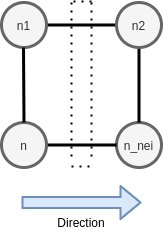
\includegraphics[scale=0.65]{rapport/valid_walls1.png}
    \caption{Représentation des noeuds pour la détermination des murs}
    \label{fig:valid_walls1}
\end{figure}

Tout d'abord, si une de ces deux arêtes n'existent pas,nous abandonnons car le mur n'est pas posable. Ensuite, l'une des difficultés est de récupérer les noeuds \texttt{n1} et \texttt{n2} car les arêtes peuvent être coupées, ce qui impliquerait que \texttt{graph\_\_get\_neighboor} nous renverrait \fbox{-1}. Nous avons choisi, au lieu d'ajouter "en dur" au noeud \texttt{n} une certaine valeur en fonction de la taille du graphe et de la direction, d'implémenter dans la structure joueur un graphe supplémentaire \texttt{naked\_graph}. Il représente le graphe à l'état initial, c'est à dire sans aucun mur posé et ne sera jamais modifié. \\

\textbf{Remarque :} Si pour chaque client, nous devons créer une copie, il n'y a qu'un seul graphe nu dans le serveur, à l'image du graphe central unique. Ce choix coûte un certain espace mais garantit la portabilité du code. \\

Pour récupérer \texttt{n1} et \texttt{n2}, nous vérifions premièrement l'élimination du mur si l'un des deux noeuds est en dehors du graphe. Ici la valeur \fbox{-1} ne peut être dû qu'à une sortie de graphe puisque c'est \texttt{naked\_graph} qui est étudié. \\

Ensuite, nous récupérons les noeuds \texttt{n1} et \texttt{n2} à partir des autres sur le vrai graphe actuel en fonction des différents cas présentés par la figure~\ref{fig:valid_walls_get}.

\begin{figure}[ht]
    \centering
    \begin{subfigure}{.5\textwidth}
        \centering
        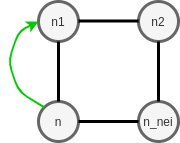
\includegraphics[width=0.6\linewidth]{rapport/valid_walls_get1.png}
        \caption{Situation 1 pour récupérer le noeud \texttt{n1}}
        \label{fig:valid_walls_get1}
    \end{subfigure}%
    \begin{subfigure}{.5\textwidth}
        \centering
        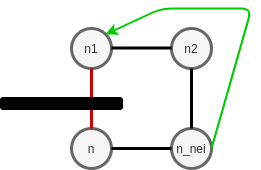
\includegraphics[width=0.75\linewidth]{rapport/valid_walls_get2.png}
        \caption{Situation 2 pour récupérer le noeud \texttt{n1}}
        \label{fig:valid_walls_get2}
    \end{subfigure}
    
    \caption{Différentes situations pour récupérer le noeud \texttt{n1}}
    \label{fig:valid_walls_get}
\end{figure}

Si, en revanche, les arêtes \texttt{(n~-~n1)} et \texttt{(n\_neighboor~-~n2)} sont coupées, comme dans la figure~\ref{fig:valid_walls_prob}, alors \texttt{naked\_graph} est réutilisé pour les obtenir. Ainsi donc, tout les cas triviaux sont maintenant traités et nous avons toujours accès aux noeuds \texttt{n1} et \texttt{n2}. Seul le cas où les arêtes \texttt{(n~-~n1)} et \texttt{(n\_neighboor~-~n2)} sont coupées n'est pas résolvable directement avec cette implémentation. En effet, simplement en regardant l'état des arêtes et des noeuds, nous ne pouvons savoir si nous sommes dans le cas d'un mur posable ou non. \\

\clearpage
\begin{figure}[ht]
    \centering
    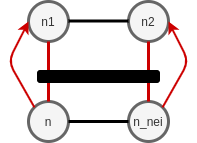
\includegraphics[scale=0.75]{rapport/valid_walls_problem.png}
    \caption{Cas problématique des arêtes \texttt{(n - n1)} et \texttt{(n\_neighboor - n2)} coupées}
    \label{fig:valid_walls_prob}
\end{figure}

Dans la figure~\ref{fig:valid_walls_trouble}, nous cherchons à déterminer si nous pouvons poser un mur entre les arêtes (6-7) et (10-11). Dans les diagrammes~\ref{fig:valid_walls2} et \ref{fig:valid_walls3}, les arêtes (6-10) et (7-11) sont coupées et pourtant les résultats sont différents. \\

\begin{figure}[ht]
    \centering
    \begin{subfigure}{.5\textwidth}
        \centering
        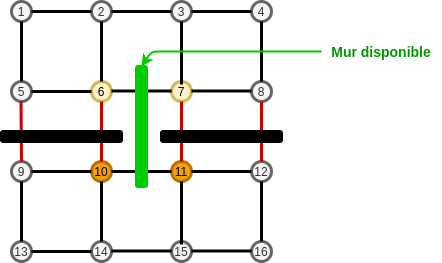
\includegraphics[width=1\linewidth]{rapport/valid_walls2.png}
        \caption{Intercalation de mur}
        \label{fig:valid_walls2}
    \end{subfigure}%
    \begin{subfigure}{.5\textwidth}
        \centering
        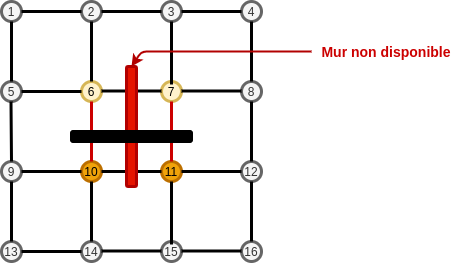
\includegraphics[width=1\linewidth]{rapport/valid_walls3.png}
        \caption{Mur impossible}
        \label{fig:valid_walls3}
    \end{subfigure}
    
    \caption{Différentes configurations où les les arêtes \texttt{n - n1} et \texttt{n\_neighboor - n2} sont coupées}
    \label{fig:valid_walls_trouble}
\end{figure}

Pour différencier ces cas, nous attribuons à chaque case entre 4 noeuds un nombre, comme représenté dans la figure~\ref{fig:valid_walls4}. Nous ajoutons à la structure \texttt{player} un tableau d'entier \texttt{wall\_installed} qui indique pour chacune de ces cases si un mur est déjà installé. Il n'y a pas besoin de mettre une valeur entière précise, pour indiquer la direction par exemple, car dès lors qu'un mur potentiellement viable est étudié, nous avons déjà vérifié qu'un mur dans le même sens n'existe pas (en vérifiant l'existence des arêtes \texttt{(n~-~n\_nei)} et \texttt{(n1~-~n2)}). \\


\begin{figure}[ht!]
    \centering
    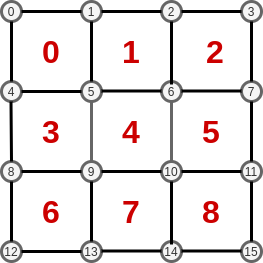
\includegraphics[scale=0.75]{rapport/valid_walls4.png}
    \caption{Numérotation des cases}
    \label{fig:valid_walls4}
\end{figure}

Pour récupérer le numéro de case, nous appelons les fonctions \texttt{min\_node}, qui détermine le noeud avec la plus faible \texttt{id} (le noeud correspond au coin gauche de la case) en fonction des 4 noeuds passés en paramètre, et la fonction \texttt{position\_square} qui renvoie le résultat de la formule~\eqref{eq:pos_square}.

\begin{equation}
    position = min\_node - (min\_node \% n) 
    \label{eq:pos_square}
\end{equation}

Ainsi donc, on vérifie que nous ne sommes pas dans le cas~\ref{fig:valid_walls3} en examinant à la bonne position le tableau \texttt{wall\_installed}. La valeur \fbox{0} signifie qu'il n'y a pas de mur, la valeur \fbox{1} qu'il y en a un. Dans ce dernier cas, on ignore le mur. \\

A partir d'ici, nous sommes capables de déterminer si un mur est posable ou non en fonction des noeuds, des arêtes et des murs déjà installés. Il suffit ensuite de boucler l'algorithme sur tous les noeuds dans toutes les directions soit une complexité O(4$n^2$) avec n la taille du graphe. Pour s'assurer qu'un mur déjà intégré au tableau de \fbox{MOVE\_T} \texttt{walls} n'est pas ajouté, la fonction \texttt{wall\_in\_list} est appelée. Cette fonction compare pour chacun des murs du tableau, le mur étudié en prenant soin de bien vérifier l'égalité de murs par la fonction \texttt{compare\_walls}. Celle-ci compare soigneusement chacun des murs en utilisant la fonction \texttt{edge\_equal} qui elle-même vérifie soigneusement l'égalité entre deux arêtes. \\

Cette vérification des murs n'est toutefois pas suffisante. En effet, il faut maintenant vérifier que lorsqu'un mur est posé, les deux joueurs ont toujours au moins un chemin viable pour atteindre une position gagnante. \\

\subsubsection{Murs qui n'entravent pas les chemins des joueurs}

C'est la fonction \texttt{existPath\_Player} qui en fonction d'une couleur et d'une position permet de savoir si il existe un chemin pour un joueur. La fonction prends également en paramètre un joueur pour avoir accès au graphe, à la liste des positions gagnantes, etc... (voir Algorithme~\ref{algo:existPath}).

\begin{lstlisting}[caption = {Spécification de la fonction déterminant l'existence d'un chemin}, label = {algo:existPath}, float = h]
int existPath_Player(struct player* p, enum color_t color, size_t pos)
\end{lstlisting}

La fonction est un algorithme de parcours en largeur qui commence la recherche de chemin à partir de la position \texttt{pos}. Dès lors, les voisins de ce noeud sont étudiés et nous traitons un noeud parmi la liste à traiter. A chaque fois qu'un nouveau noeud est traité, il est marqué par le biais d'un tableau d'entier où \fbox{0} correspond à un noeud non marqué et \fbox{1} un noeud marqué. Nous pouvons résumer ce processus par la suite d'exemple de la figure~\ref{fig:parcours_graphe}. \\

Dans cet exemple, les noeuds en attente sont représentés en bleu et les noeuds considérés comme \texttt{marqués} sont représentés en violet. Les positions gagnantes pour un joueur sont quant à elles colorées en vert. \\

\clearpage

\begin{figure}[ht]
    \centering
    \begin{subfigure}{.5\textwidth}
        \centering
        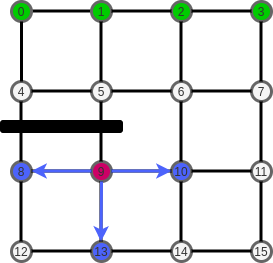
\includegraphics[scale=0.7]{rapport/parcours_graphe1.png}
        \caption{Etat initial}
        \label{fig:parcours_graphe1}
    \end{subfigure}%
    \begin{subfigure}{.5\textwidth}
        \centering
        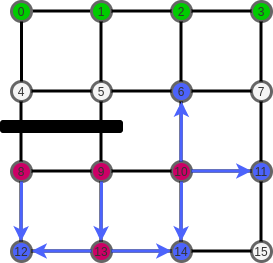
\includegraphics[scale=0.7]{rapport/parcours_graphe2.png}
        \caption{Etat après 4 noeuds traités}
        \label{fig:parcours_graphe2}
    \end{subfigure}%
    
    
    
    \begin{subfigure}[b]{.5\textwidth}
        \centering
        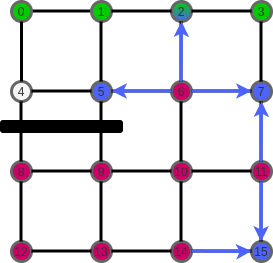
\includegraphics[scale=0.7]{rapport/parcours_graphe3.png}
        \caption{Etat après 8 noeuds traités}
        \label{fig:parcours_graphe3}
    \end{subfigure}%
    \begin{subfigure}[b]{.5\textwidth}
        \centering
        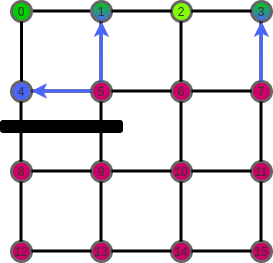
\includegraphics[scale=0.7]{rapport/parcours_graphe4.png}
        \caption{Etat après 12 noeuds traités}
        \label{fig:parcours_graphe4}
    \end{subfigure}%

    \caption{Simulation d'un parcours en largeur}
    \label{fig:parcours_graphe}
\end{figure}




Ensuite, Nous vérifions à chaque fois si le noeud qu'on traite correspond à une position gagnante en fonction de la couleur. On peut donc désormais vérifier s'il existe un chemin pour un joueur. \\

Finalement, pour vérifier si un mur peut être posé, il suffit de :
\begin{enumerate}
    \item Poser le mur sur le graphe local
    \item Vérifier que le joueur \fbox{WHITE} a un chemin vers une case noire
    \item Vérifier que le joueur \fbox{BLACK} a un chemin vers une case blanche
    \item Détruire le mur
    \item Ajouter ou ne pas ajouter le mur aux murs légaux en fonction des résultats (2) et (3) \\
\end{enumerate}

La fonction \texttt{checkPath} s'occupe de ce processus. Sur l'exemple~\ref{fig:check_path1}, nous pouvons observer les différents chemins possibles pour les deux joueurs. Tant que les deux joueurs ont au moins un chemin encore possible, le mur étudié est légal. Nous obtenons donc pour ce même exemple, le schéma~\ref{fig:check_path2} des murs légaux et illégaux.

\begin{figure}[ht!]
    \centering
    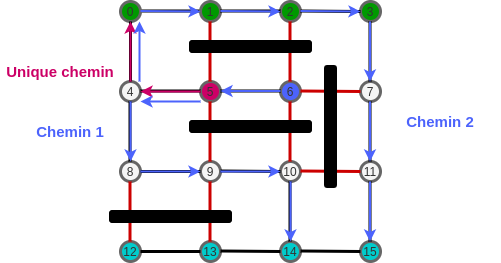
\includegraphics[scale=0.7]{rapport/check_path1.png}
    \caption{Chemins disponibles pour chacun des joueurs}
    \label{fig:check_path1}
\end{figure}

\begin{figure}[ht!]
    \centering
    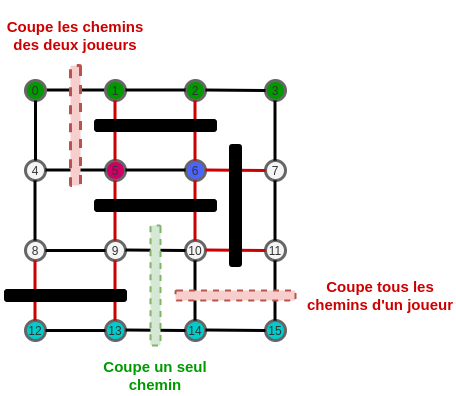
\includegraphics[scale=0.7]{rapport/check_path2.png}
    \caption{Murs légaux et illégaux}
    \label{fig:check_path2}
\end{figure}

\clearpage  
\section{Implémentation des stratégies des joueurs}

Si, à ce stade du développement, nous avons déjà deux joueurs qui récupèrent aléatoirement un coup autorisé, il faut maintenant implémenté des réelles stratégies pour que les clients commencent à gagner. Les fonctions dites "stratégiques" sont implémentées dans le fichier \fbox{strategy.c}.

\subsection{Implémentation d'une stratégie naïve}

La première stratégie implémentée vise à diriger le joueur vers une position gagnante. Il est donc censé courir le plus rapidement possible en ligne droite. Pour cela, nous définissons une variable \texttt{gap} qui se calcule de la façon suivante (équation~\eqref{eq:gap}):

\begin{equation}
    gap = \lvert position\_gagnante - position\_joueur \rvert
    \label{eq:gap}
\end{equation}

Le joueur \fbox{Rick J-19 Z7} cherche alors à trouver le mouvement qui réduira au minimum cette valeur. Cette implémentation permet d'ordonner les mouvements de façon hiérarchique (voir figure~\ref{fig:rush1}).

\begin{figure}[ht]
    \centering
    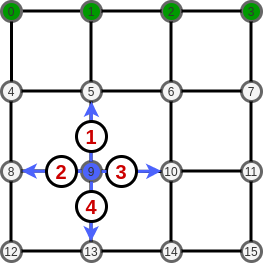
\includegraphics[scale=0.65]{rapport/rush1.png}
    \caption{Ordre de préférence des mouvements par le joueur \fbox{Rick J-19 Z7}}
    \label{fig:rush1}
\end{figure}

Cela reste une stratégie naïve. En effet, dans le cas d'une impasse, le joueur sera incapable de l'esquiver. (voir figure~\ref{fig:rush2}). Il restera donc indéfiniment coincé dedans, alternant un mouvement en avant et un mouvement en arrière. \\

\begin{figure}[h!t]
    \centering
    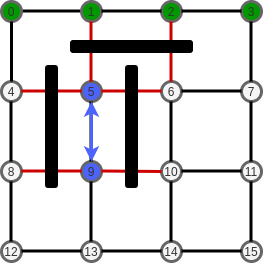
\includegraphics[scale=0.65]{rapport/rush2.png}
    \caption{Joueur \fbox{Rick J-19 Z7} bloqué indéfiniment}
    \label{fig:rush2}
\end{figure}

Cette stratégie n'est donc pas convaincante. Ce problème est lié au fait que le joueur n'a qu'une vision basique du plateau de jeu, il ne comprends pas qu'il peut contourner le problème en reculant 2 fois avant de se décaler sur le côté et d'avancer.

\subsection{Implémentation d'une stratégie convaincante}

La stratégie \textit{intelligente} que nous souhaitons implémenter correspond à une stratégie intuitive dite "double Dijkstra". Elle vise à calculer le plus court chemin d'un joueur mais également celui de son adversaire. Si son chemin est plus court, le joueur avance. Dans le cas contraire, il pose un mur bloquant son adversaire et rallongeant son chemin.

\subsubsection{Algorithme Dijkstra}
L'algorithme du plus court chemin est l'algorithme Dijkstra. Si l'algorithme de base permet de récupérer un plus court chemin pour atteindre un noeud, nous souhaitons dans notre cas qu'il étudie un ensemble de positions victorieuses. \\

Tout d'abord, nous avons définit une structure \texttt{node} qui contient l'\texttt{id} d'un noeud, la variable \texttt{predecessor} qui lie un noeud à son prédécesseur et la variable \texttt{dist} qui donne la distance du noeud par rapport à la position. Précisement, la variable \texttt{predecessor} est un entier qui correspond à la position du noeud prédécesseur dans le tableau \texttt{nodes}. Cette structure est très pratique car, dès lors qu'une position gagnante est trouvée, il suffit de récupérer les prédécesseurs pour obtenir le plus court chemin (exemple figure~\ref{fig:predecessor}. \\

\begin{figure}[ht]
    \centering
    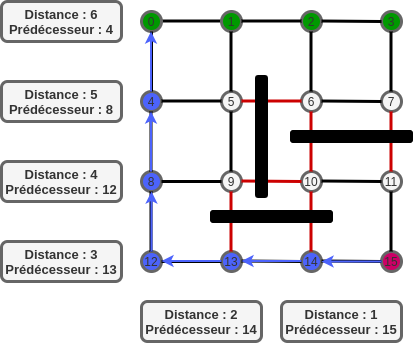
\includegraphics[scale=0.7]{rapport/predecesseurs.png}
    \caption{Schéma des prédécesseurs}
    \label{fig:predecessor}
\end{figure}

Étant donné que nous souhaitons utilisé cet algorithme pour chacun des joueurs à l'intérieur d'un seul client, nous donnons tout les arguments utiles plutôt que de simplement passer la structure \texttt{player} (voir Algorithme~\ref{algo:dijkstra}). 
D'où le prototype de la fonction :

\begin{lstlisting}[caption = {Spécification de la fonction dijkstra}, label = {algo:dijkstra}, float = h]
struct moves_valids* dijkstra(struct graph_t* graph, size_t n, size_t pos, size_t ennemy_pos, enum color_t c, size_t* winning_nodes, size_t numb_win);
\end{lstlisting}

L'algorithme de Dijkstra est très semblable au parcours en largeur que nous avons explicité plus haut, la seule différence étant que nous traitons des \texttt{nodes} plutôt que des \texttt{id}. Lorsqu'une position gagnante est trouvée, la fonction \texttt{get\_predecessor}, qui fabrique le chemin, est appelée. Le dernier élément correspond à la position gagnante atteinte tandis que le premier élément correspond à la position \texttt{pos} du joueur. \\

\subsubsection{Algorithme intelligent de pose de mur}

Nous souhaitons gêner l'adversaire dès lors qu'il a un chemin plus court que notre propre chemin. C'est la fonction \texttt{cut\_ennemy\_path} qui se charge de retourner le meilleur mur. Selon notre définition propre, le meilleur mur est un mur qui augmente la distance parcourue par le joueur adverse, qui ne coupe pas le propre chemin du joueur et qui est le plus proche du camp du joueur. Ce dernier critère peut paraître surprenant, pourtant il est plutôt logique. Si on pose des murs en face du joueur adverse, on risque d'être gêner plus tard par ce même mur. \\

Premièrement, nous avons implémenté la fonction qui vérifie que notre propre chemin n'est pas coupé. C'est \texttt{is\_cutting\_path} qui se charge de cette vérification. Elle vérifie qu'il n'y a aucune égalité entre les deux noeuds d'une future arête coupée et deux noeuds relié par le meilleur chemin. Si c'est le cas, c'est que notre propre chemin est coupé par ce mur. Ainsi donc, cela permet à notre joueur de poser le mur convenablement comme dans la figure (~\ref{fig:cut_path1}) plutôt que celui de l'exemple (~\ref{fig:cut_path2}). \\

\begin{figure}[ht]
    \centering
    \begin{subfigure}{.5\textwidth}
        \centering
        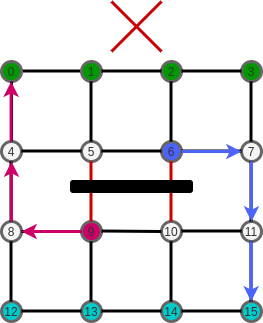
\includegraphics[scale=0.7]{rapport/cut_path.png}
        \caption{Mur qui coupe notre chemin}
        \label{fig:cut_path1}
    \end{subfigure}%
    \begin{subfigure}{.5\textwidth}
        \centering
        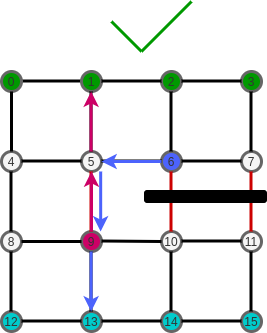
\includegraphics[scale=0.7]{rapport/cut_path2.png}
        \caption{Mur qui ne coupe pas notre chemin}
        \label{fig:cut_path2}
    \end{subfigure}%

    \caption{Placement de mur sans autoblocage}
    \label{fig:cut_path}
\end{figure}




Ensuite, puisque nous cherchons à poser des murs le plus proche de notre camp plutôt que en face du joueur adverse, nous étudions les noeuds traversés par le joueur adverse en partant de la fin. Dès que nous trouvons un mur posable qui rallonge le temps adverse et qui ne coupe pas notre chemin, nous savons que c'est le "meilleur mur". \\

Finalement, nous appelons la fonction \texttt{double\_dijkstra\_strategy} qui calcule les deux chemins pour les joueurs et décide de renvoyer un mouvement ou un mur en fonction des cas. Elle appelle toutes les fonctions cités plus haut et résume la stratégie de notre joueur \fbox{Rick D. Sanchez III}. \\

\textbf{Remarque :} Si nous sommes sûr de perdre la partie, par exemple s'il n'y a plus de mur posable qui coupe le joueur adverse, alors le programme renvoie le mouvement trouvé par l'algorithme Dijkstra afin de maintenir l'intégrité du jeu.

\subsubsection{Amélioration par le calcul}

Notre stratégie précédente reste \textit{hasardeuse}. En effet, elle part du principe que le meilleur mur correspond au premier mur intéressant, c'est à dire le mur le plus proche du bord qui rallonge le temps adverse sans rallonger notre propre temps. Sauf qu'il est tout à fait possible qu'il y ait un meilleur mur, qui soit certes plus éloigné de notre camp, mais qui allonge plus significativement le trajet adverse (exemple figure \ref{fig:cut_path_best_wall}). Cet exemple est apparu être une cause majeure de défaites dans nos parties contre les autres équipes sur le \texttt{ladder}. Nous avons tout de même décidé de garder notre joueur \fbox{Rick D. Sanchez III} et avons donc implémenté un nouveau joueur, \fbox{Rick C-137}. \\

\begin{figure}[ht!]
    \centering
    \begin{subfigure}{.5\textwidth}
        \centering
        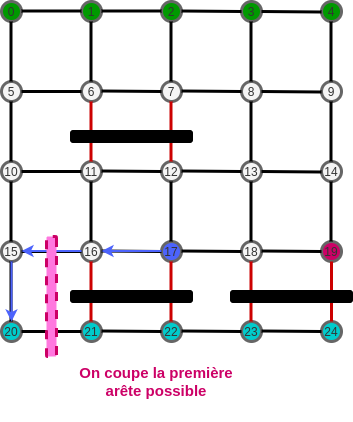
\includegraphics[scale=0.6]{rapport/cut_path3.png}
        \caption{Mur le plus proche du bord}
        \label{fig:cut_path3}
    \end{subfigure}%
    \begin{subfigure}{.5\textwidth}
        \centering
        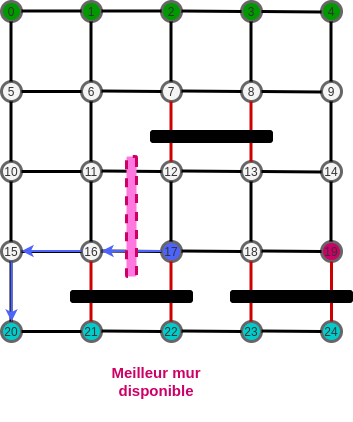
\includegraphics[scale=0.6]{rapport/cut_path4.png}
        \caption{Mur qui allonge le plus le chemin adverse}
        \label{fig:cut_path4}
    \end{subfigure}%

    \caption{Définitions diverses du meilleur mur}
    \label{fig:cut_path_best_wall}
\end{figure}


Pour remédier à ce problème, nous avons décidé de véritablement calculer ce meilleur mur. La fonction \texttt{find\_best\_wall} correspond à ce calcul. Elle est découpée en 2 étapes majeures. \\

\begin{enumerate}
    \item \textbf{Récupérer les murs intéressants} \\
Dans un premier temps, la fonction \texttt{fill\_wall\_array} remplit une structure \texttt{moves\_valids} avec les murs intéressants. Ces murs sont les murs qui coupent le chemin du joueur adverse, calculé avec l'algorithme Dijkstra. \\ 

\textbf{Remarque :} Nous pourrions tout à fait étudier tout les murs, qui pour rappel sont déjà calculés par \texttt{valid\_walls}. Cependant, ce ne serait pas optimal (très forte complexité) et il n'y a que pour concevoir des "pièges" qu'il y a un intérêt à étudier les murs qui ne rallongent pas immédiatement le trajet adverse. Notre joueur n'étant pas dans cette catégorie, nous préférons nous limiter aux murs coupant le chemin obtenu. \\

La fonction est assez similaire à \texttt{cut\_ennemy\_path}, le programme itère en partant de la fin sur les noeuds traversés par le chemin du joueur adverse. Ensuite chacun des murs possibles est stocké par la fonction \texttt{add\_wall\_by\_vertex} qui vérifie systématiquement que le mur est légal. Nous pouvons résumer cette idée par la figure \ref{fig:cut_path5}. Nous faisons remarquer que puisque les murs légaux ont tous été calculés, nous faisons une simple recherche dans notre structure \texttt{walls}. \\ 

\begin{figure}[h!]
    \centering
    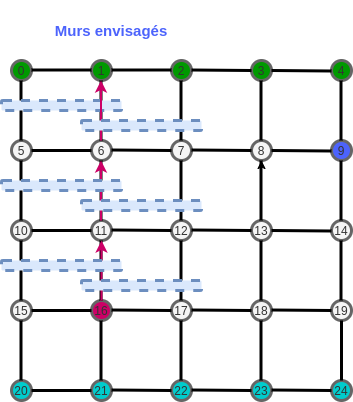
\includegraphics[scale=0.6]{rapport/cut_path5.png}
    \caption{Murs intéressants envisagés}
    \label{fig:cut_path5}
\end{figure}

Un seul cas problématique apparaît avec cette implémentation. Lorsqu'il y a un saut sur un joueur adverse, il n'est pas possible de créer un mur entre les deux noeuds étudiés (voir figure \ref{fig:cut_path6}). Nous devons donc sous découper le problème en deux, d'abord en étudiant l'arête \texttt{(noeud destination / position joueur)} et ensuite l'arête \texttt{(position joueur / noeud de départ)}.  Nous identifions le problème en vérifiant si l'arête existe via \texttt{graph\_\_edge\_exists} pour obtenir le résultat figure \ref{fig:cut_path7}. Nous sommes donc à ce stade certain de récupérer tous les murs intéressants. Il faut maintenant pouvoir calculer le meilleur. \\

\clearpage
\begin{figure}[ht!]
    \centering
    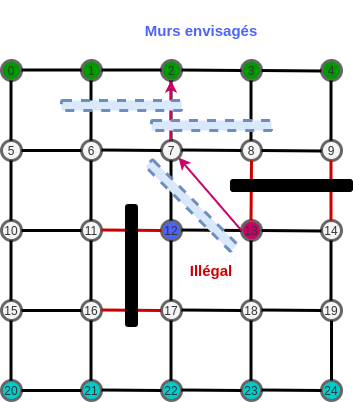
\includegraphics[scale=0.7]{rapport/cut_path6.png}
    \caption{Tous les murs intéressants non trouvés}
    \label{fig:cut_path6}
\end{figure}

\begin{figure}[ht!]
    \centering
    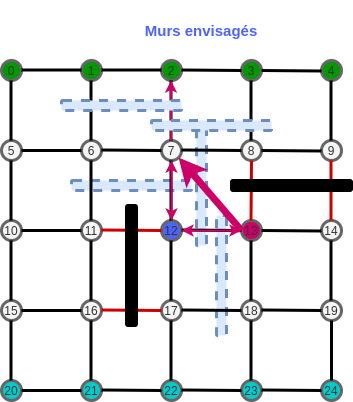
\includegraphics[scale=0.7]{rapport/cut_path7.png}
    \caption{Tous les murs intéressants trouvés}
    \label{fig:cut_path7}
\end{figure}

    \item \textbf{Calculer le meilleur mur} \\
C'est la fonction \texttt{super\_\_study\_gap} qui se charge de récupérer le meilleur mur. Tout d'abord, nous arrêtons de vérifier que le mur ne coupe pas notre chemin. En effet, il peut exister des cas où poser un mur sur notre chemin allonge plus encore le chemin adverse (exemple \ref{fig:study_gap1} avec le mur bleu qui rajoute 2 mouvements à l'adversaire rose contre seulement 1 pour le joueur bleu.). \\
    
\begin{figure}[ht!]
    \centering
    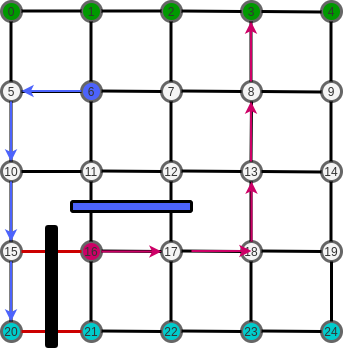
\includegraphics[scale=0.6]{rapport/study_gap1.png}
    \caption{Exemple de pose de mur intelligente}
    \label{fig:study_gap1}
\end{figure}

Pour donc ne négligez aucun cas, nous posons le mur étudié, et étudions la différence par la variable \texttt{gap} entre les longueurs des chemins des joueurs et nous retirons le mur. On garde en mémoire le mur qui maximise \texttt{strictement} la variable \texttt{gap}. Étant donné que nous étudions les murs dans l'ordre dans lequel ils ont été remplis par \texttt{fill\_wall\_array}, c'est à dire en partant par les plus proches noeuds du camp du joueur, nous récupérons donc à la fois \textbf{le meilleur mur} en terme de différence de taille entre les chemins mais également \textbf{le plus proche mur du camp du joueur} s'il y en a plusieurs. \\

\textbf{Remarque :} A l'initialisation, nous calculons la situation actuelle via \texttt{initial\_gap}. Comme précédemment, s'il n'y a aucun mur qui améliore la situation, c'est à dire en augmentant la différence entre les chemins du joueur et de son adversaire, alors le programme le mouvement trouvé par l'algorithme Dijkstra.
    
\end{enumerate}
 
 
 \subsection{Une nouvelle approche stratégique}
 
 Dans l'optique de construire un joueur toujours plus performant, une autre approche a été envisagée en parallèle, moins calculatoire mais plus réfléchie. Notre but a été de prendre du recul sur le classement compétitif, et d'en tirer des conclusions pour bâtir une stratégie convaincante. Un tel joueur n'a cependant pas vu le jour du fait de la complexité algorithmique de certains composants de sa stratégie, ainsi nous avons préféré passer du temps sur sa conception et son algorithme, plutôt que sur l'implémentation de ces derniers (qui aurait pu être faite avec plus de temps). \\
 
Le pseudo-algorithme de ce joueur est trouvable dans le fichier \texttt{player\_rick\_evil}. et nous nous y référerons par la suite par le nom \fbox{Evil Rick}.

\subsubsection{Processus de conception}

Quitte à évoluer dans un environnement compétitif, il nous a semblé important d'observer nos adversaires. En étudiant les parties des autres joueurs sur le \texttt{ladder}, nous nous sommes rendus compte qu'une grande partie des joueurs hauts dans le classement utilisaient des algorithmes de plus court chemin pour décider de leur avance, et agir en faisant "confiance" à leur résultat. L'autre partie, quant à elle, optait pour une prise de possession du plateau en construisant un dédale de murs jusqu'à s'assurer le contrôle du terrain. \\

Pour contrecarrer ces deux principales façons d'agir, il nous fallait donc une stratégie permettant de laisser la première catégorie agir comme si elle pouvait gagner (afin que les algorithmes de pose de murs ne soient pas trop sollicités) et de poser quelques murs au centre du plateau pour s'assurer un chemin rapide vers la sortie. Après un peu de réflexion, nous avons eu l'idée de se battre principalement contre le premier type de joueur, en espérant que les effets collatéraux contrecarreraient le second. \\

Ainsi, il a été décidé de mettre en défaut les algorithmes de plus court chemin, comme Dijkstra : puisque nos adversaires sont des programmes avec des stratégies limitées, ils ne "voient" pas le plateau avec du recul. L'installation d'un piège bien placé pourrait ainsi leurrer les joueurs dans une direction qu'un humain aurait très vite détecté comme un piège évident. \\

Nous avons alors effectué diverses recherches sur des ouvertures classiques\cite{openings} du Quoridor, en étudiant celles qui conviendraient à notre type de piège. Notre dévolu s'est porté sur une version altérée de l'ouverture dite de \textbf{"Quick Box"}\cite{quickbox}. Cette ouverture n'est pas considérée comme très "efficace" en temps normal car elle laisse beaucoup de liberté à un joueur humain qui comprend le subterfuge assez vite, et ainsi elle est habituellement utilisée pour contrôler la position du joueur adverse tôt dans la partie. \\

Cependant, sa forte simplicité venant de la séparation des chemins du joueur adverse en un virtuellement plus court mais piégé (voir figure~\ref{fig:quickbox}), et un autre plus long, en a fait le candidat idéal pour une implémentation suffisamment peu complexe. 

\clearpage
\begin{figure}[ht]
    \centering
    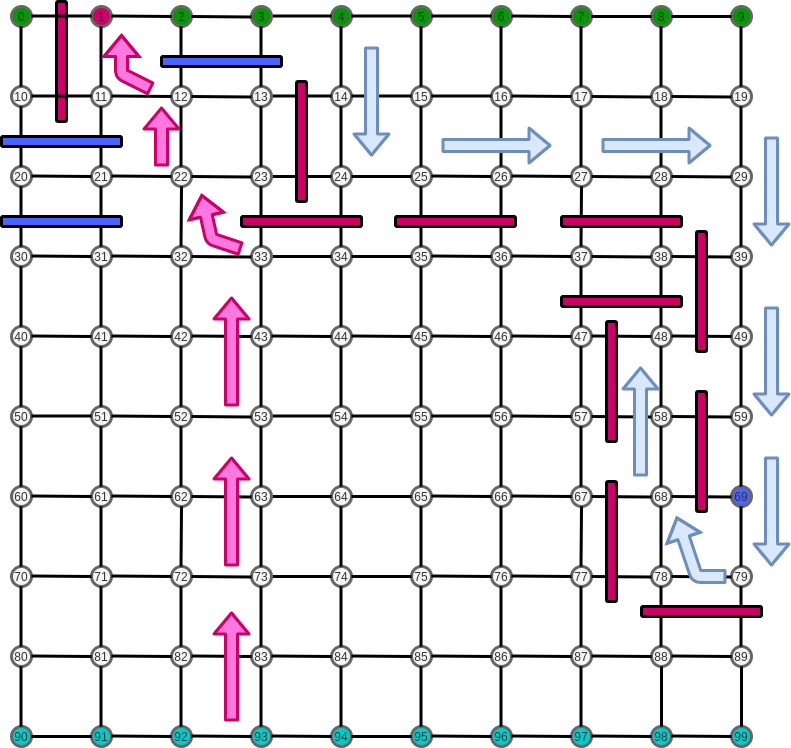
\includegraphics[scale=0.5]{rapport/white_mage2.png}
    \caption{Exemple simulé d'une partie avec le joueur \fbox{Evil Rick}}
    \label{fig:quickbox}
\end{figure}

\subsubsection{Écriture de l'algorithme}

Ainsi (voir figure~\ref{fig:trapsetup}), cette stratégie consiste à poser un mur, dès nos premiers tours de jeu, qui va diviser le plateau en deux parties : un "cul-de-sac", et une "sortie". Là où un joueur humain serait sorti du cul de sac rapidement, notre but va être de leurrer le programme adverse dans un couloir toujours plus long, en le persuadant à chaque étape qu'il est en avance. Un instant avant sa victoire, il sera alors temps de "refermer le piège", et alors son plus court chemin vers une position gagnante va se rallonger de dizaines de cases. Pour rendre le leurre plus performant encore, notre algorithme n'hésite pas à se bloquer lui-même en "gaspillant" un mur, pour appâter l'algorithme adverse en faisant pencher les calculs de distance en sa faveur dans le cas où nous serions à égalité.\\

\begin{figure}[ht]
    \centering
    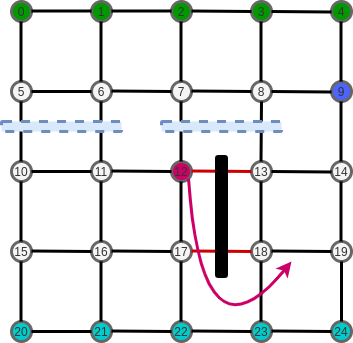
\includegraphics[scale=0.7]{rapport/white_mage1.png}
    \caption{Ouverture par le joueur \fbox{Evil Rick}}
    \label{fig:trapsetup}
\end{figure}

Notre algorithme se repose sur la définition en interne de ces fameuses zones de cul de sac et de sortie, ce qui représente un défi en terme de programmation puisque ces zones sont "abstraites", et leur position dépend de beaucoup de facteurs (position de départ adverse, murs gênants entravant le piège, taille du plateau). Bien que nous n'ayons pas pu écrire les fonctions gérant ces zones par manque de temps, nous avons défini tout le protocole à suivre pour en reproduire le comportement. De ce fait, la plupart des éléments pouvant perturber la stratégie ont été pris en compte, et une réponse adaptée leur a été trouvée, ce qui résulte en un arbre de décision massif à multiples embranchements dans le pseudo-algorithme. \\

Le bon déroulement de l'opération repose donc sur quatre étapes :

\begin{itemize}
    \item \textbf{Placer le mur diviseur} lorsque le joueur adverse avance pour la première fois.
    \item Tant qu'il est dans la zone de la \texttt{quick box}, tenter d'\textbf{agrandir cette zone en largeur}.
    \item Une fois qu'il ne reste plus qu'un couloir de 1 ou 2 de large pour passer, \textbf{approfondir ce couloir} pour laisser le joueur adverse se rapprocher de l'arrivée.
    \item Lorsqu'il est suffisamment proche, \textbf{refermer le couloir} pour fermer le piège et le regarder faire tout le chemin inverse.
\end{itemize}

\paragraph{}
Chacune de ces étapes nécessite de vérifier en permanence deux éléments essentiels : le premier est qu'aucune "autre" sortie n'existe que celle définie par la \texttt{quick box}, sans quoi le piège est caduc. On peut vérifier une telle assertion en appliquant un parcours en profondeur du graphe depuis le cul de sac en ayant bouché la sortie. Le second et plus important est qu'il n'existe pas de moyen de bloquer la sortie. Sinon, il suffirait à l'adversaire de bloquer cette sortie pour s'assurer que le piège ne puisse pas être fermé (car seul chemin possible) et obtenir la victoire sans soucis. \\

L'avantage de notre stratégie est qu'elle nous laisse du temps pour agir et nous adapter : chaque mur placé pour rallonger le cul de sac nous laisse un "tour supplémentaire". Ce temps doit impérativement être mis à profit pour empêcher la fermeture de la sortie du piège (par des murs placés en travers, par exemple), et s'assurer un trajet vers les positions gagnantes. Ainsi, lorsque l'adversaire se retrouvera piégé, son nombre de possibilités de rallonger notre propre chemin aura été limité au maximum. Dans le cas où de telles précautions n'auraient pas été prises, nous nous retrouverions avec peu de murs disponibles, une rentabilisation des murs très faible, et un adversaire possédant la majorité de ses murs et tout l'espace qu'il désire pour les rentabiliser. La défaite serait inévitable. \\

Paradoxalement, le meilleur moyen de mettre à mal cette stratégie est de se bloquer soi-même. En s'entravant avec des murs bien placés, ou en bloquant des sorties "inutiles" aux yeux d'un algorithme n'ayant pas de regard sur le plateau, le piège peut rapidement être déconstruit et la situation se retourner en notre défaveur. Si tel est le cas, on en revient alors aux stratégies classiques (voir la section précédente). Au vu des parties testées contre des ordinateurs en ligne, il apparaît aussi que tenter de bloquer la sortie tôt dans la partie (en utilisant sa supériorité en nombre de murs disponibles) semble la stratégie la plus efficace pour l'adversaire.

 

\section{Tests}

Les tests sont segmentés de la même manière que les fichiers sources, c'est à dire que chaque fichier \fbox{*.c} a son fichier \fbox{test\_*.c}. Les tests sur les graphes ont également différents tests, des tests structurels et fonctionnels. On sépare également les tests de création de type de graphe (carré, serpent, etc.) dans le fichier \fbox{alltests.c}.

\subsection{Tests de graphes}
\subsubsection{Tests de manipulation de graphes}
Les fonctions de manipulation de graphes sont testées de différentes manières, via des tests fonctionnels et des tests structurels. À chaque fonction est attribuée une batterie de tests, pour vérifier d'un coté le résultat renvoyé par la fonction, et d'un autre coté les modifications effectuées sur la matrice d'adjacence du graphe. L'ajout d'une arête entre deux sommets met à jour correctement la matrice d'adjacence, la bonne valeur est placée et l'arête est créée dans les deux sens, d'un sommet $i$ vers $j$ et inversement. \\

De même lors d'un enlèvement d'arête, les bonnes valeurs doivent être remises à zéro. D'un autre côté, nous testons le fait qu'une arête ne peut être enlevée ou créée deux fois, mais peut être à nouveau ajoutée ou retirée, respectivement. Des tests similaires sont effectués sur l'ensemble des autres fonctions de manipulation de graphe afin de vérifier la cohérence de nos fonctions. Ces tests ont été réalisés assez tôt dans l'avancement du projet, ce qui nous a permis d'avoir une base saine et fiable pour modifier les graphes à notre guise, notamment pour la création de graphes spécifiques. \\

Le but de ces tests est principalement de vérifier tous les cas complexes ou non-standards, et de s'assurer que nos fonctions réagissent comme nous le voulons à chaque fois. Ainsi, les problèmes dans la suite du projet viendront presque assurément des fonctions de plus haut niveau, puisque nous serons sûrs de celles constituant notre socle de base. 

\subsubsection{Tests sur la forme des graphes}
Afin d'avoir un plateau de jeu de la bonne forme nous avons testé les graphes pour différentes tailles.
Tout d'abord le graphe carré est testé pour différentes tailles par une fonction, et de plus la matrice d'adjacence manuellement lors de la création de la fonction qui génère le graphe a également été vérifiée. Quant aux autres formes de plateau, les matrices d'adjacences sont testées relativement à une référence qui est la matrice d'adjacence d'un graphe carré de même taille. Grâce à cette méthode nous avons seulement besoin de calculer les sommets qui sont retirés du graphe carré pour obtenir le graphe actuel, et vérifier que les seules différences entre ces deux graphes sont les liaisons avec les sommets mentionnés précédemment. De cette manière, nous avons pu testé le graphe torique et le graphe haché pour les tailles 3, 6 et 9, et, le graphe serpent pour les tailles 5 et 10.

\subsubsection{Tests relatifs aux murs}
Nous vérifions dans ces tests que les règles sont biens respectées quant au placement des murs.
Entre autre, un mur déjà placé ne peut pas être placé à nouveau, un mur ne peut pas en couper un autre et un chemin existe entre la position des joueurs et une position gagnante chacun. Pour ce faire, deux joueurs sont positionnés sur un plateau de jeu de taille 5 puis nous posons des murs progressivement tout en faisant des tests à chaque étape. La fonction qui permet de placer des murs est testée séparément, pour vérifier qu'un mur peut être placé, puis que les arêtes du graphes sont retirées et qu'un mur ne peut pas être placé là où il n'y a pas d'arête.

\subsection{Tests des coups et des stratégies}

Compte tenu de l'implémentation des fonctions des fichiers \fbox{utils.c} et \fbox{strategy.c}, on ne peut qu'envisager des tests fonctionnels. En effet, les fonctions sont généralement liés et donc dépendantes entre elles. \\

Voici comment sont organisés les tests : \\
Chaque fonction a une liste commentée des tests effectués (voir Algorithme~\ref{algo:tests}) et un message indiquant chaque étape importante (Pose ou destruction d'un mur, téléportation d'un joueur, etc.). Ensuite, si l'option \texttt{verbose} \fbox{-v} a bien été passé en argument, on obtient le descriptif complet des tests avec une information sur leur validation ou non (figure~\ref{fig:tests_verbose}). \\

\begin{lstlisting}[caption = {Tests décris pour la fonction \texttt{valid\_positions()}}, label={algo:tests}]
/* Tests made for function valid_positions()
 *
 * Player in a corner
 * Player in the center
 * Player in the center in front of the ennemy player
 * Player in the center in front of the ennemy player and wall in front
 * Player in the center in front of the ennemy player and wall in front + wall on right side
 * Player in the center in front of the ennemy player and wall in front + walls on sides
 *
 */
\end{lstlisting}

\begin{figure}[ht]
    \centering
    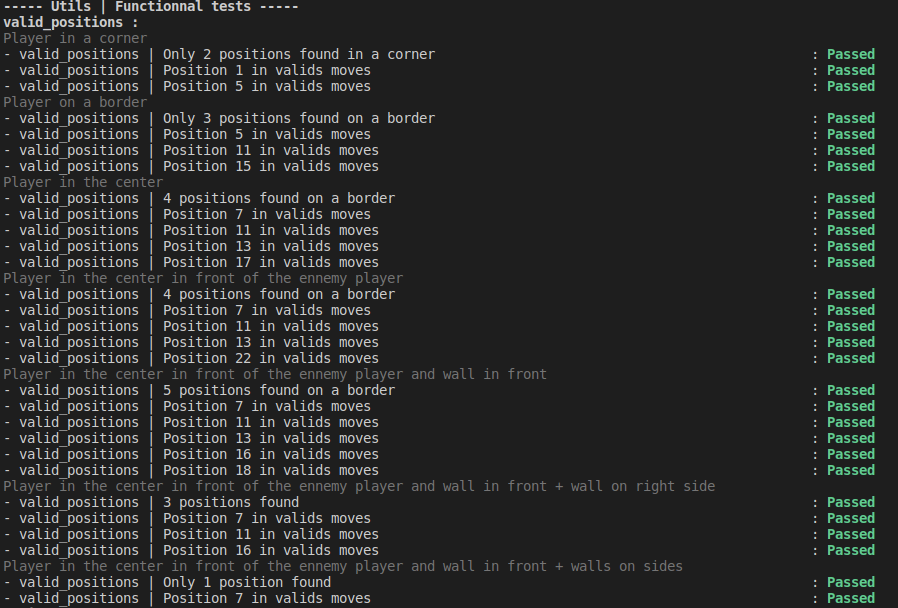
\includegraphics[scale=0.5]{rapport/tests_valid.png}
    \caption{Tests complets de \texttt{valid\_positions}}
    \label{fig:tests_verbose}
\end{figure}

Ces tests garantissent l'intégrité des fonctions avec des exemples non triviaux, surtout pour les fonctions les plus complexes (\texttt{valid\_positions}, \texttt{valid\_walls} et \texttt{dijkstra}).

\subsection{Gestion de la mémoire}

Le client et les serveurs ont été codés en gardant en tête la notion de mémoire. Ainsi, \texttt{valgrind} a été utilisé tout au long du projet pour s'assurer qu'il n'y ait pas de fuites mémoires, et le projet rendu en est exempt (tous les blocs alloués sont bien rendus). \\

A l'utilisation de \texttt{valgrind} sur notre serveur, le nombre de blocs alloués pourrait paraître important (25.000 allocations pour un plateau de taille 10), mais le programme ne prend pas autant de place à l'exécution. Nous nous sommes en effet appuyés sur la norme \textbf{ANSI~C} pour le code, et tous les éléments des tableaux sont initialisés dynamiquement (là où la norme C99 permettait une initialisation statique). Ainsi, chaque élément alloué est libéré très rapidement après, et presque aucun élément ne reste alloué l'entièreté de la partie.

\section{Conclusion}

\subsection{Apports techniques}
\paragraph{}
Pour conclure, notre implémentation du serveur ainsi que des différents clients est cohérente avec les demandes du sujet. L'utilisation des matrices creuses de la bibliothèque dynamique de \texttt{GSL} n'a pas été évidente aux premiers abords, mais après le temps d'adaptation nécessaire à sa compréhension, nous avons réussi à nous en servir correctement. En ce qui concerne la création et l'utilisation de bibliothèques dynamiques, le manuel d'utilisation de la bibliothèque \texttt{dlfcn} est relativement facile à comprendre et nous avons su mettre en place cette solution pour nos clients.

\paragraph{}
Comme notre implémentation des graphes mais aussi des méthodes de calcul nécessaires aux joueurs est conséquente, son équivalent en tests l'est aussi. Bien que notre couverture soit très convenable (99\% en tests unitaires, environ 85\% en tests d'intégration), il est nécessaire de souligner le temps non négligeable passé à écrire, tester et remodeler les tests unitaires et fonctionnels des graphes et des méthodes pour les joueurs. En effet, pour pouvoir déboguer plus facilement les graphes, nous avons mis en place une visualisation du plateau dans le terminal. Ce temps consacré à cette interface graphique nous a permis dans la suite de la réalisation des tests d'éviter de perdre du temps à ne pas comprendre un potentiel bug (d'indexage de noeuds ou de création d'arêtes par exemple).

\paragraph{}
Enfin, l'implémentation des clients est plutôt concluante, avec notre meilleur joueur \fbox{Rick C-137} dans le haut du classement. Parti depuis le bas du classement avec de nombreux bugs à corriger, nous avons réduit l'écart avec les meilleurs clients petit à petit tout au long du projet. L'affinement de nos algorithmes de calculs de choix de mouvements est plutôt satisfaisante, bien qu'il existe toujours de nombreuses améliorations. Par exemple, lui permettre d'avoir une vision plus globale du partie (Calculer les situations actuelles ainsi que les situations futures après 1 coup joué) serait une piste.  De plus, réussir à finalisé l'implémentation de \fbox{Evil Rick} pourrait être une autre piste pour commencer à avoir des stratégies bien plus complexes.

\subsection{Recul sur le travail effectué}
\paragraph{}
Ce projet nous a apporté de nouvelles connaissances tant sur la gestion d'un projet en équipe de quatre personnes et la répartition des tâches que sur les notions de développement logiciel vues en cours de Programmation impérative 2. En effet, la mise en place de tests conséquents et pertinents, la création et l'utilisation de bibliothèque dynamique, la gestion de la couverture ainsi que l'approfondissement de la compilation séparée sont des notions importantes pour la suite de notre cursus, et les appliquer dans un projet semestriel est une étape importante à passer.

\paragraph{}
Nous sommes finalement relativement satisfaits du travail que nous avons réalisé sur l'ensemble du projet, de la stabilité et de la couverture de notre implémentation. De plus, nos différents clients, réalisés ou théoriques, ont eu leur intérêt dans l'avancement du projet, tant dans un premier temps dans l'assimilation de l'environnement de travail et des bibliothèques, que dans l'approfondissement de nos algorithmes et de la recherche de solutions face à la rude compétition. Évidemment, nous aurions souhaité pouvoir finaliser notre dernier client \fbox{Evil Rick}, mais aussi pouvoir imaginer de nouvelles stratégies à implémenter.

\clearpage
\bibliographystyle{unsrt}
\bibliography{bibliography}

\end{document}